
\documentclass[12pt]{book}

\usepackage[norsk]{babel} 
\usepackage[utf8]{inputenc}
\usepackage{graphicx}
\graphicspath{ {img/} }

\begin{document}
\clearpage

\newcommand\nbvspace[1][3]{\vspace*{\stretch{#1}}}
\newcommand\nbstretchyspace{\spaceskip0.5em plus 0.25em minus 0.25em}
\newcommand{\nbtitlestretch}{\spaceskip0.6em}
\pagestyle{empty}
\begin{center}
\bfseries
\nbvspace[1]
\Huge
{\nbtitlestretch\huge
Gubberenn Dataprogram \\}

\nbvspace[10]
\normalsize

Bruksanvisning\\
GDPKonsoll\\

\nbvspace[2]

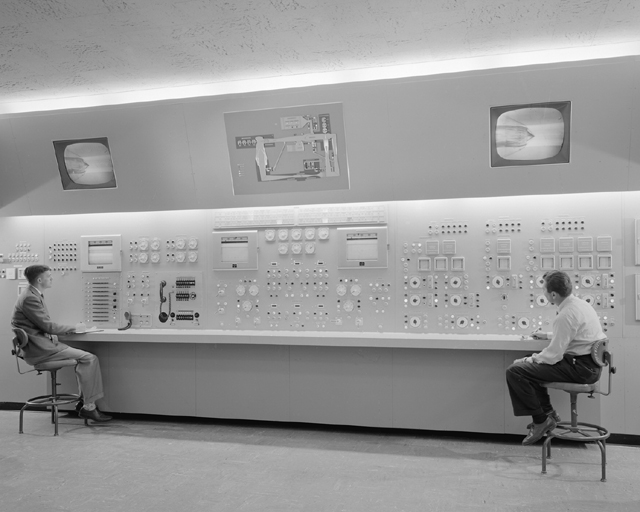
\includegraphics[width=5.0in]{datacenter}
\nbvspace[15]
\normalsize

20(C)15\\
\large
Trøbbel \& Trevare A/S
\nbvspace[1]
\end{center}

\tableofcontents

\chapter{Historikk}

Dette kapitlet tar for seg litt historikk rundt bruk av ulike dataprogram i 
forbindel med arrangeringen av Gubberennet opp gjennom tidene, og kan følgelig 
glatt hoppes over, om du kun er interessert i bruksanvisningen til 'gubb.exe'. 

\section{DataEase}

En gang for lenge siden ble det første 'gubb' -dataprogrammet laget. Vi 
snakker om 1993, eller der omkring. Det var Jan-Erik Nordahl som satte dette  
sammen ved hjelp av et verktøy som heter "DataEase for DOS". 

"DataEase for DOS" er et såkalt 4. generasjons database-vertøy. Disse verktøyene var 
ganske populære på slutten av 1980- og starten av 1990-tallet. DataEase er
dog 'in business' forsatt når dette skrives, som er våren 2015, og mange bruker faktisk 
fortsatt denne teknologien.

Følgelig kan dette 'ur-gubb' -dataprogrammet forsatt benyttes. Men på grunn av noen teknikaliteter rundt den plattformen som 
programmet fra 1993 er basert på, slikt som at det egentlig er 16 bits DOS software, fungerer koden erfaringsmessig kun opp til 
Windows XP ServicePack 3. I utgangspunktet er ikke dette noe problem, siden man kan kjøre en virtuell Windows XP på et hvilket 
som helst moderne operativsystem.

Figur 1.1 viser et bilde av dette oppsettet rundt programmet, mens figur 1.2 viser et bilde hvor DataEase-applikasjonen kjører på en virtuell 
Windows XP instans vha Oracle VM VirtualBox på en Linux-maskin. 

\begin{figure}
\centering
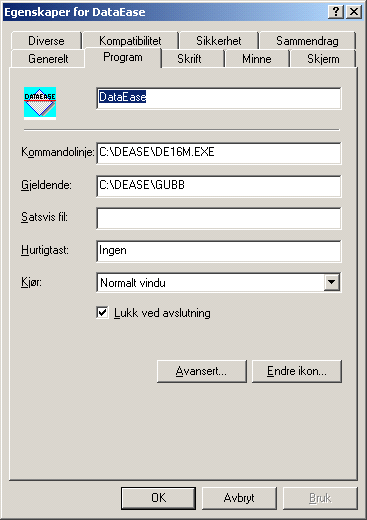
\includegraphics[width=12.0cm]{bilde}
\caption{Legg merke til  'gjeldende'}
\end{figure}

\begin{figure}
\centering
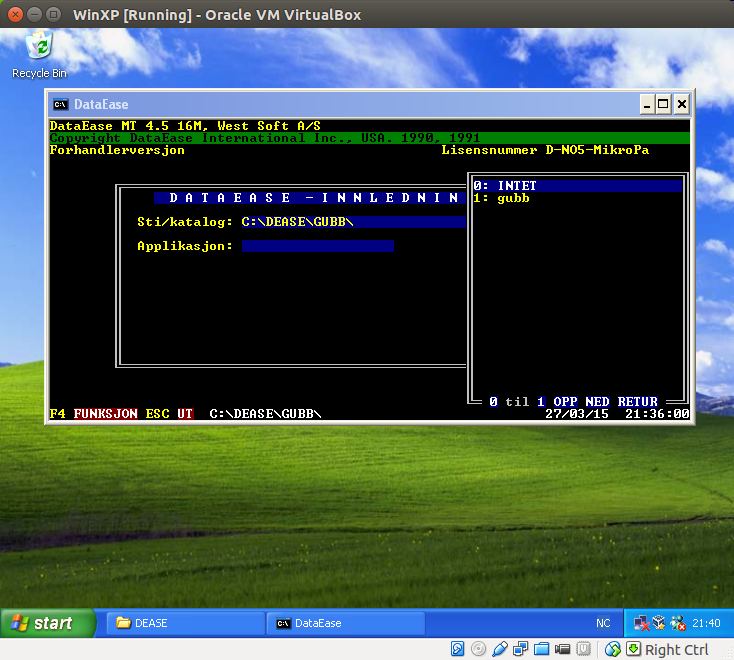
\includegraphics[width=12.0cm]{bilde_a}
\caption{DBASE på en virtuell Windows XP}
\end{figure}

\section{Programmeringsspråket C}

Programmeringsspråket jeg har valgt for å implementere en ny versjon av 'gubb', er C. Grunnen til at jeg har valgt C er fordi 
dette programmeringsspråket antageligvis er det aller mest fleksible språket man kan utvikler programmvare i. Skal man lage et enkelt dataprogram som skal kunne 
benyttes i lang tid fremover, så anser jeg C som førstevalget. Et enkelt C-program kan kompileres til å kjøre på nesten alt som 
kan tenkes på av plattformer. C er også et av de grunnleggende programmeringsspråkene, og et språk som egner seg godt som det første 
programmeringsspråket man lærer seg. Siden problemstillingene som 'gubb' løser, er enkle og lettfattlige, så kan kanskje C -koden benyttes til å lære seg litt C, for de som ønsker det. 

\chapter{Bruksanvisning}

\section{Installasjon}

\section{Registrer brukere}

\section{Registrer anvendt tid}

\section{Registrer oppgavepoeng}

\section{Utfør beregningene}

\section{Skriv ut rapporter}


\end{document}
